
	El filtro de Kalman obtiene la mejor estimación en el sentido del error cuadrático medio. Esto quiere decir que cuanto mayor sea la varianza del ruido de proceso, más importancia le dará a las mediciones. De la misma manera, cuanto mayor sea la varianza del ruido de medición, mayor importancia le dará al modelo en el espacio de estados para poder realizar la estimación. El objetivo de este Sección es ver cómo se modifica la estimación cambiando la magnitud de la matriz de covarianza del ruido de proceso.
	
	\subsection{$R^{'}\gg R$}
	
	\begin{figure}[H]
		\centering
		%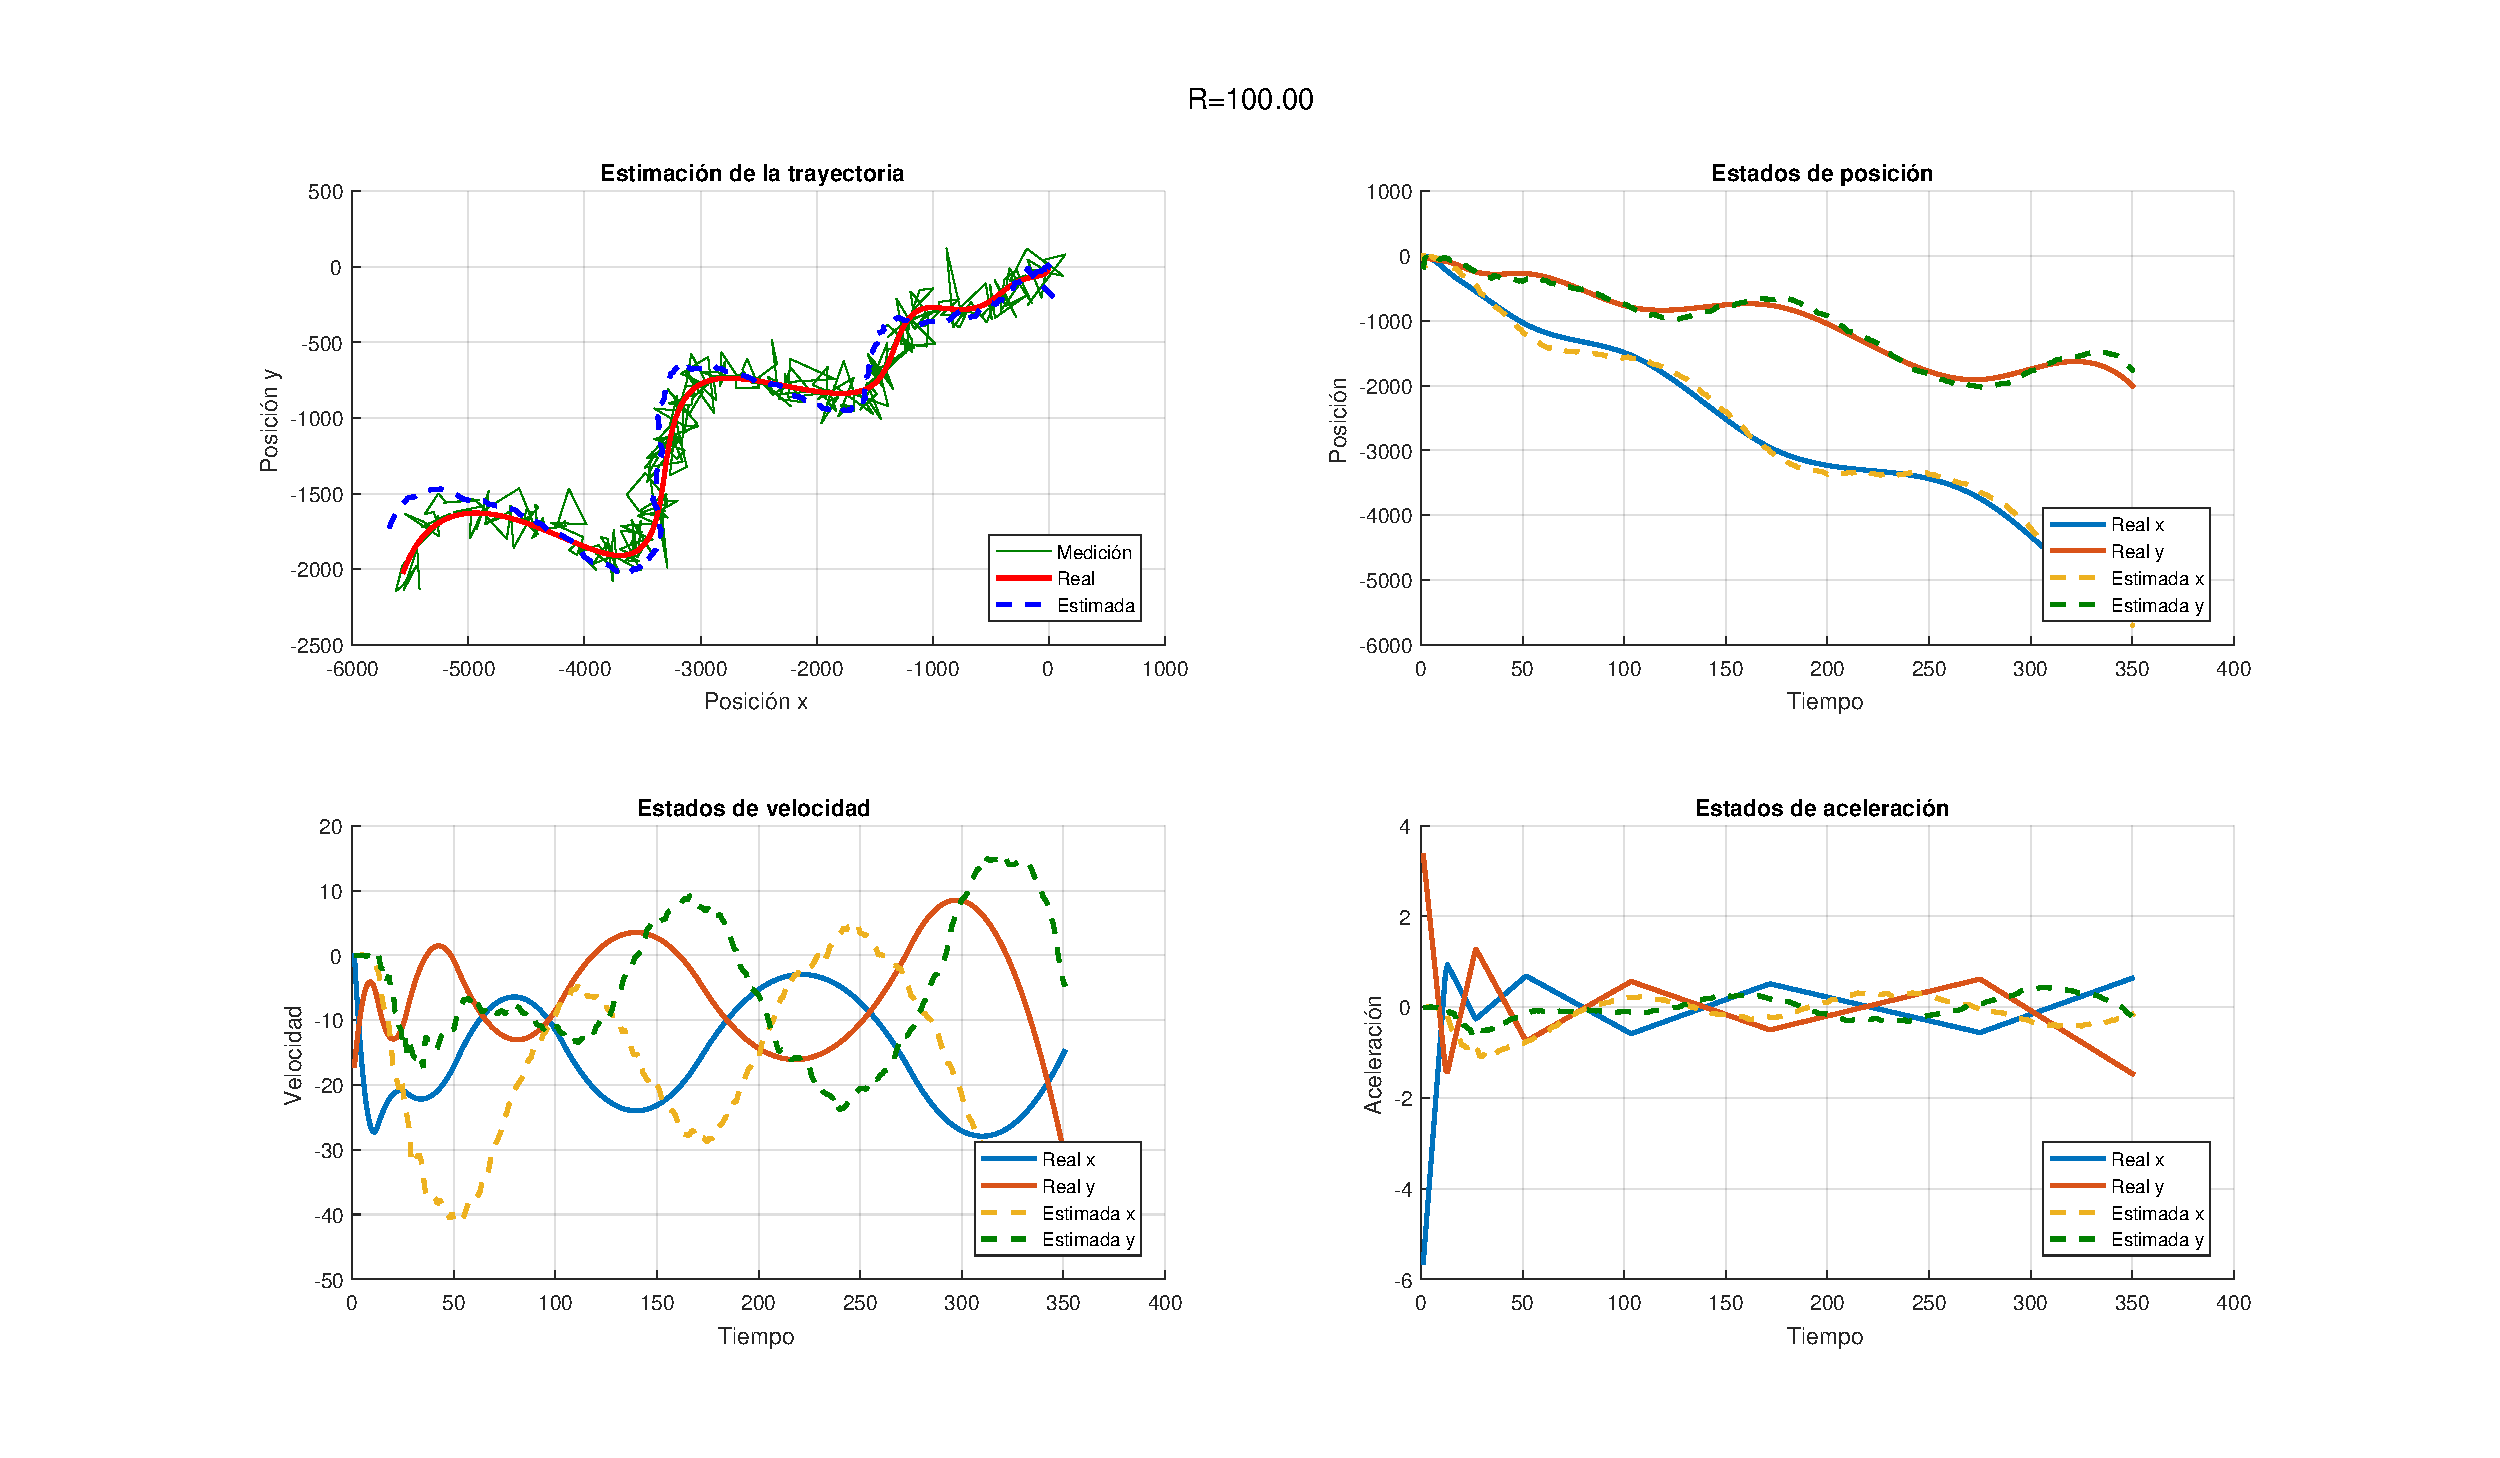
\includegraphics[width=1.0\textwidth,keepaspectratio]{Figuras/graf_ej6_R1.pdf}
		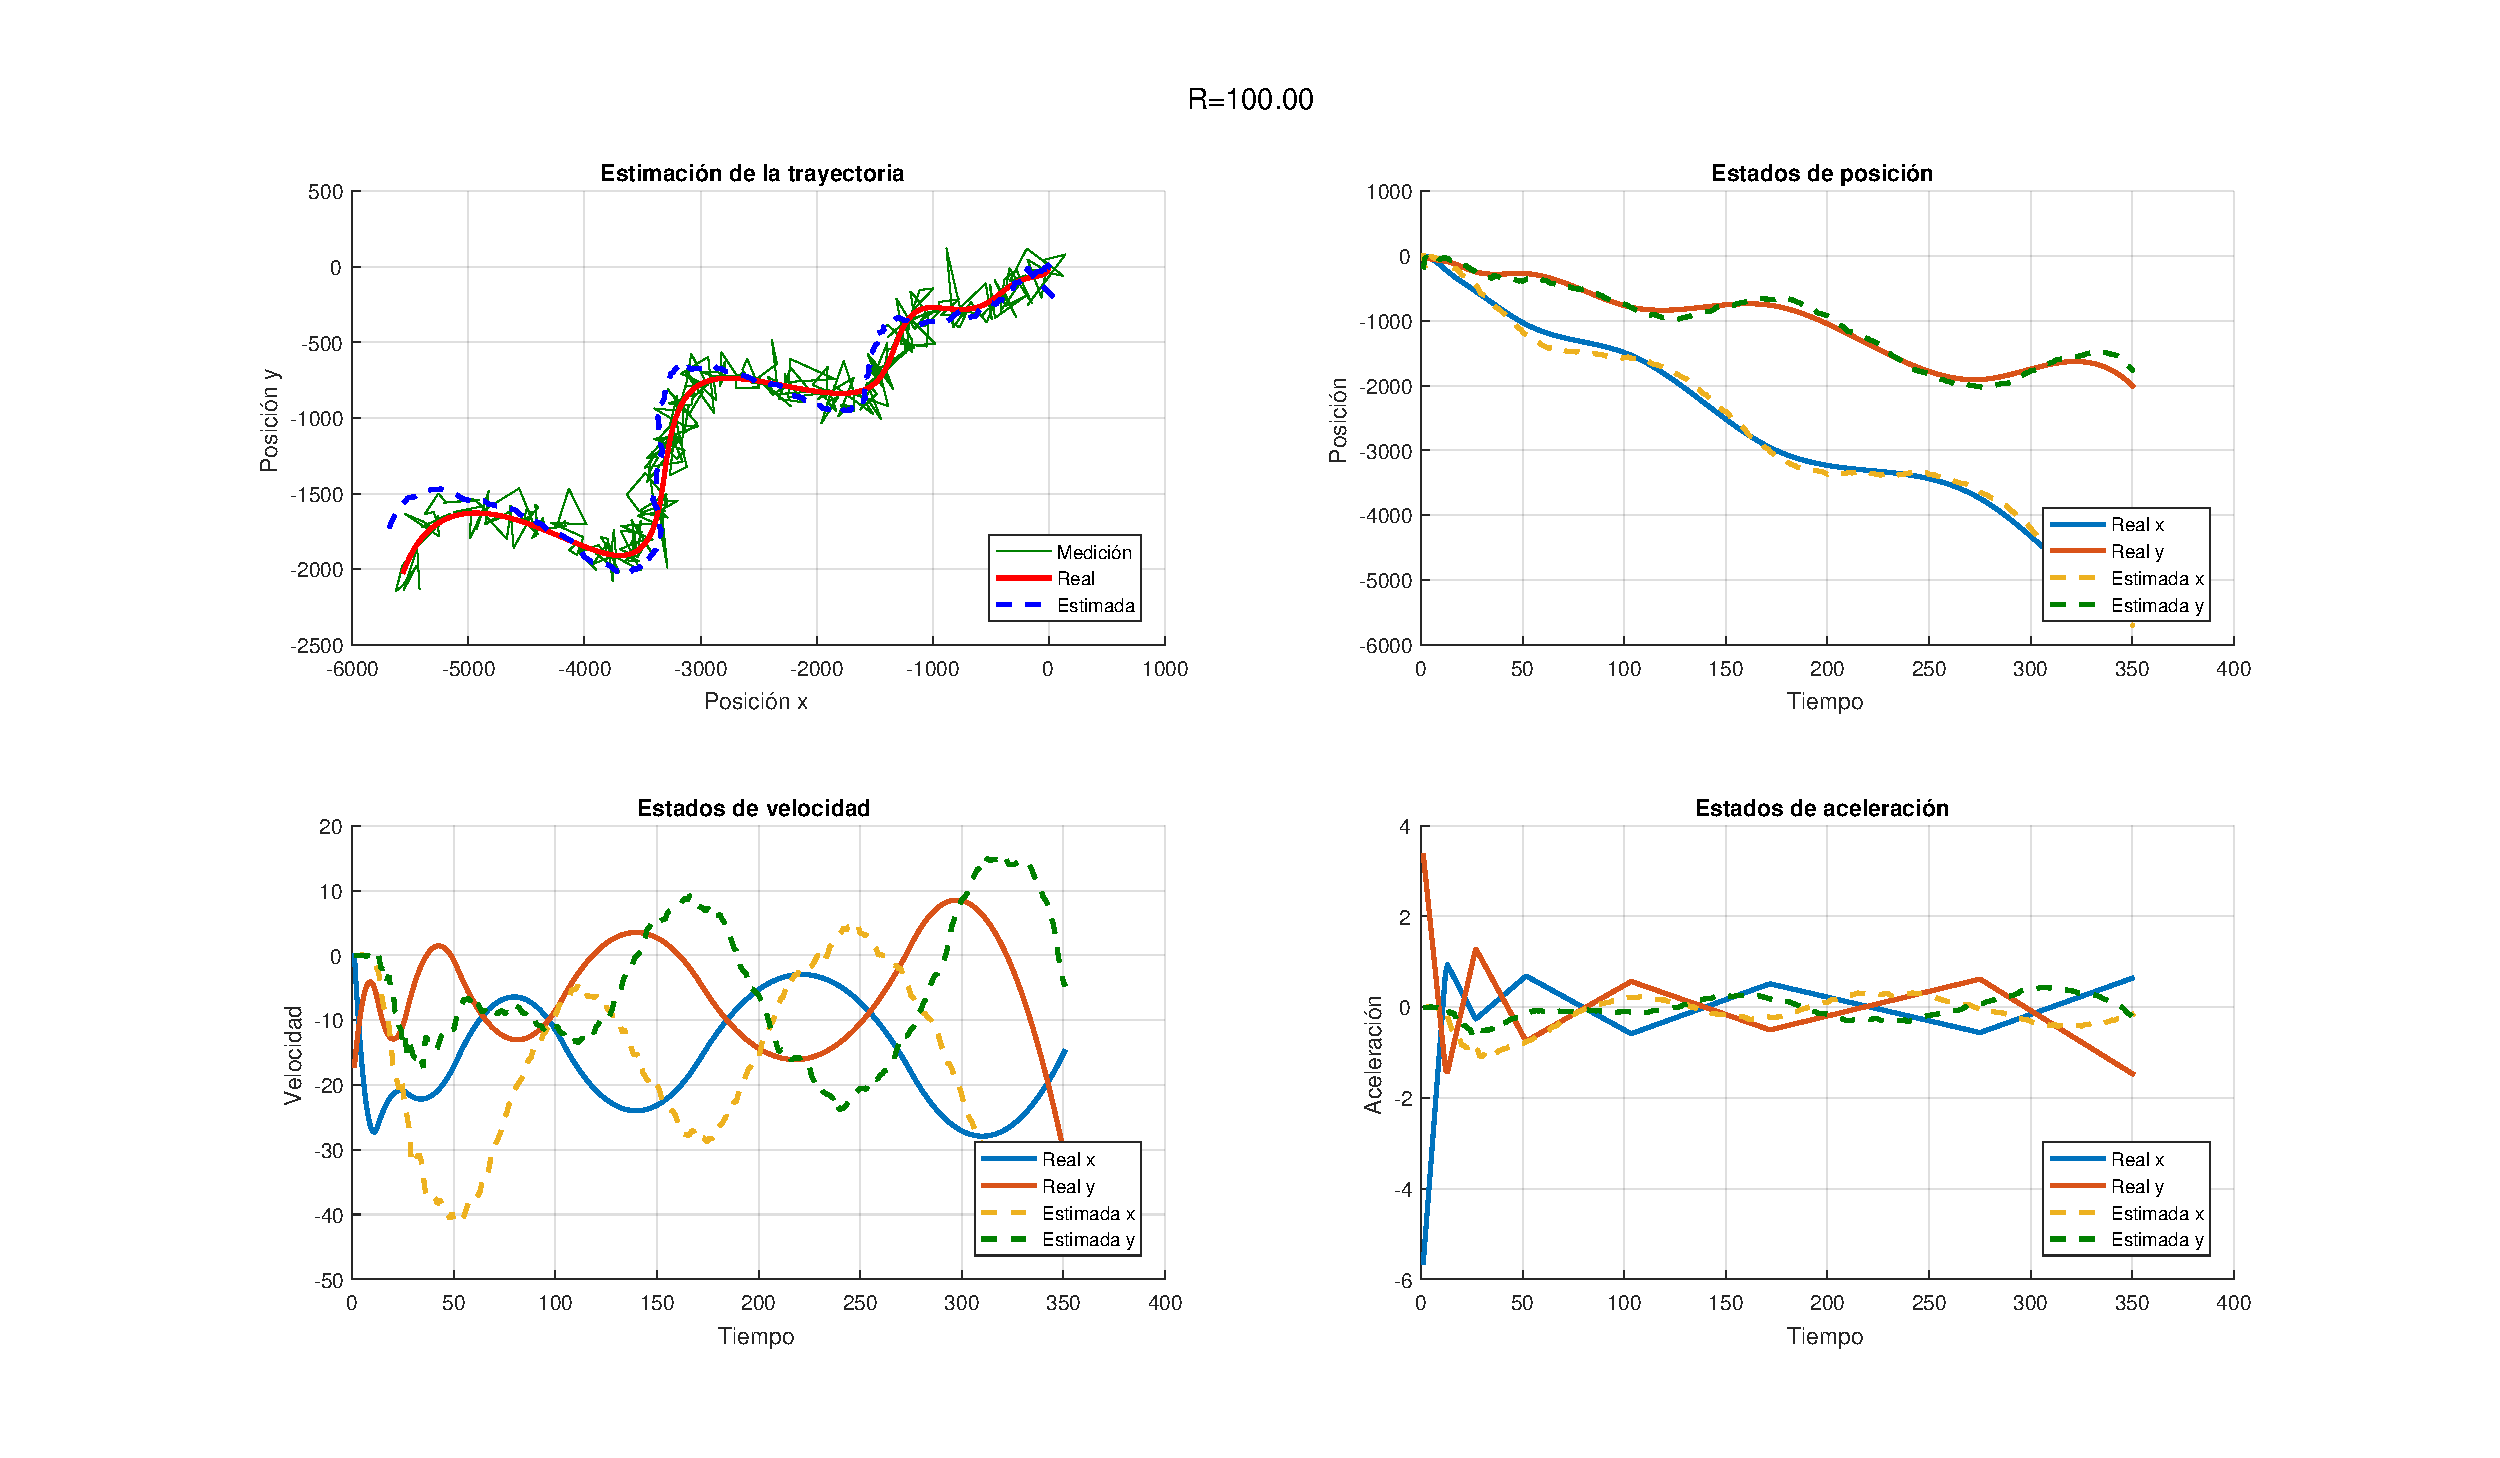
\includegraphics[scale=0.5,trim={6,5cm 0 0 0}]{Figuras/graf_ej6_R1.pdf}
		\caption{Estimación de Trayectoria - Matriz de Covarianza Mayor}
		\label{fig:ej5r1}
	\end{figure}

	\begin{figure}[H]
		\centering
		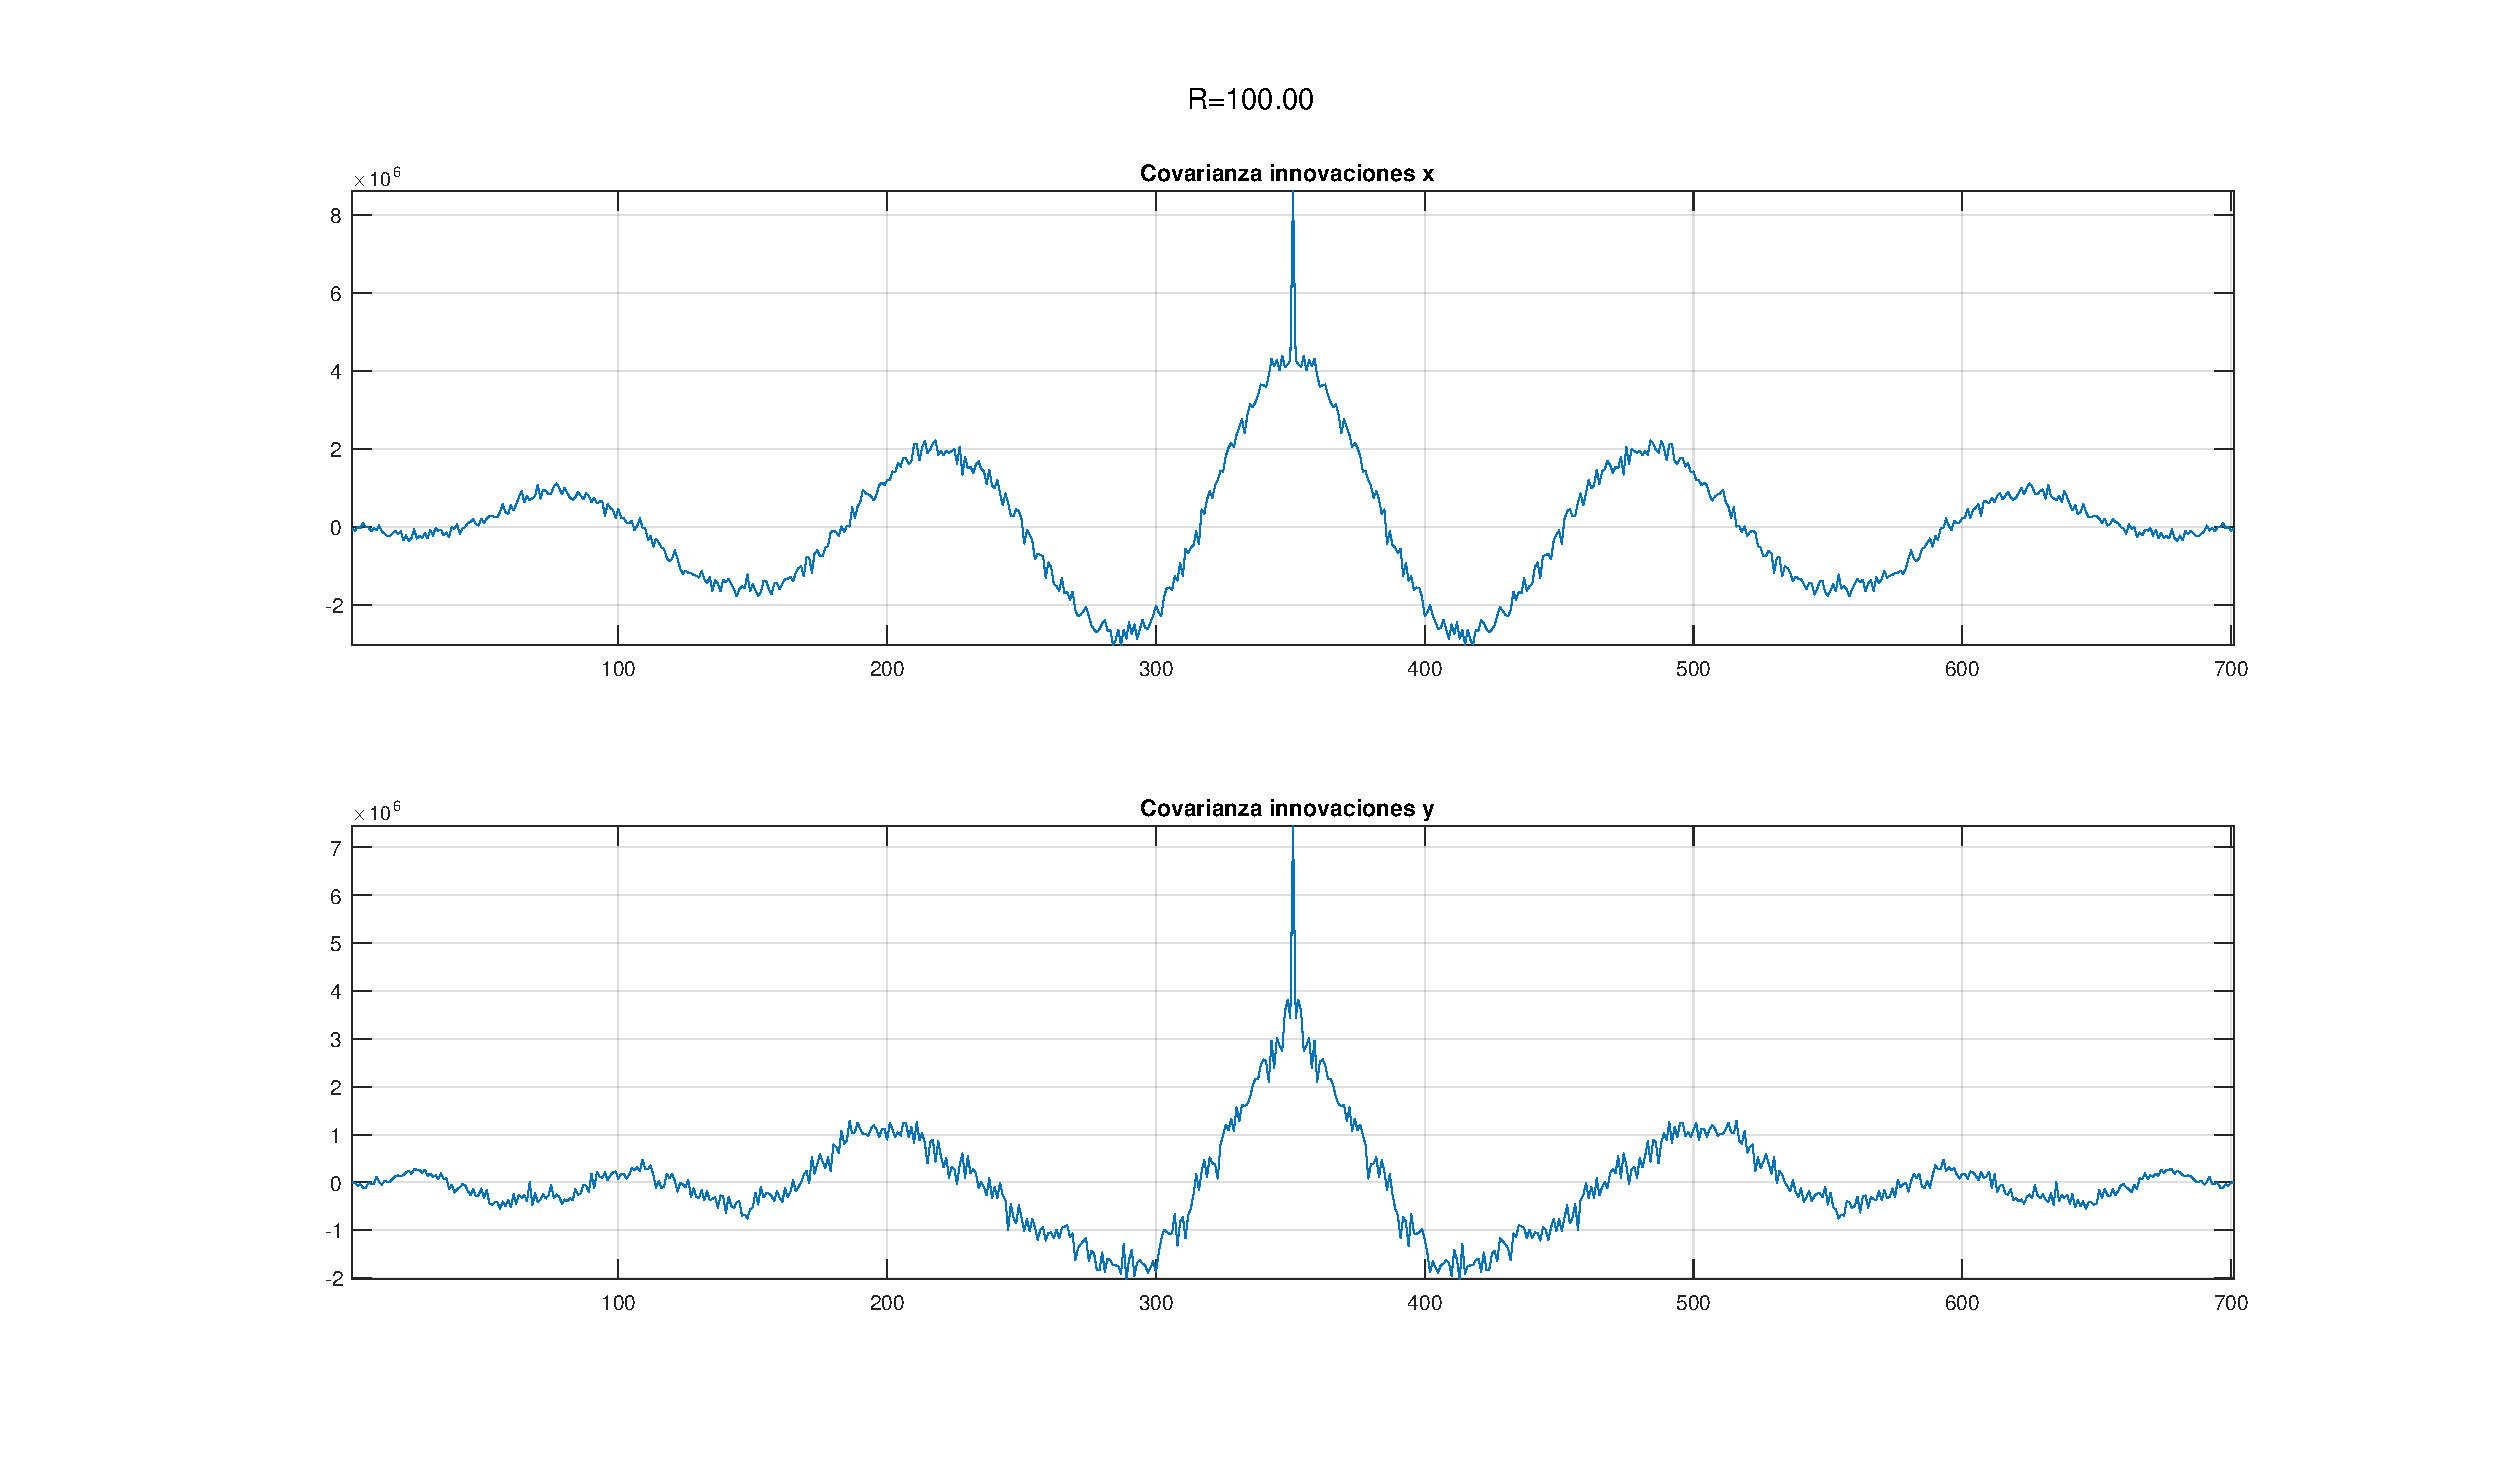
\includegraphics[width=1.0\textwidth,keepaspectratio]{Figuras/covinn_ej6_R1.pdf}
		\caption{Autocorrelación de Innovaciones - Matriz de Covarianza Mayor}
		\label{fig:ej5r1_innov}
	\end{figure}

	
	\subsection{$R^{'}\ll R$}
	
	\begin{figure}[H]
		\centering
		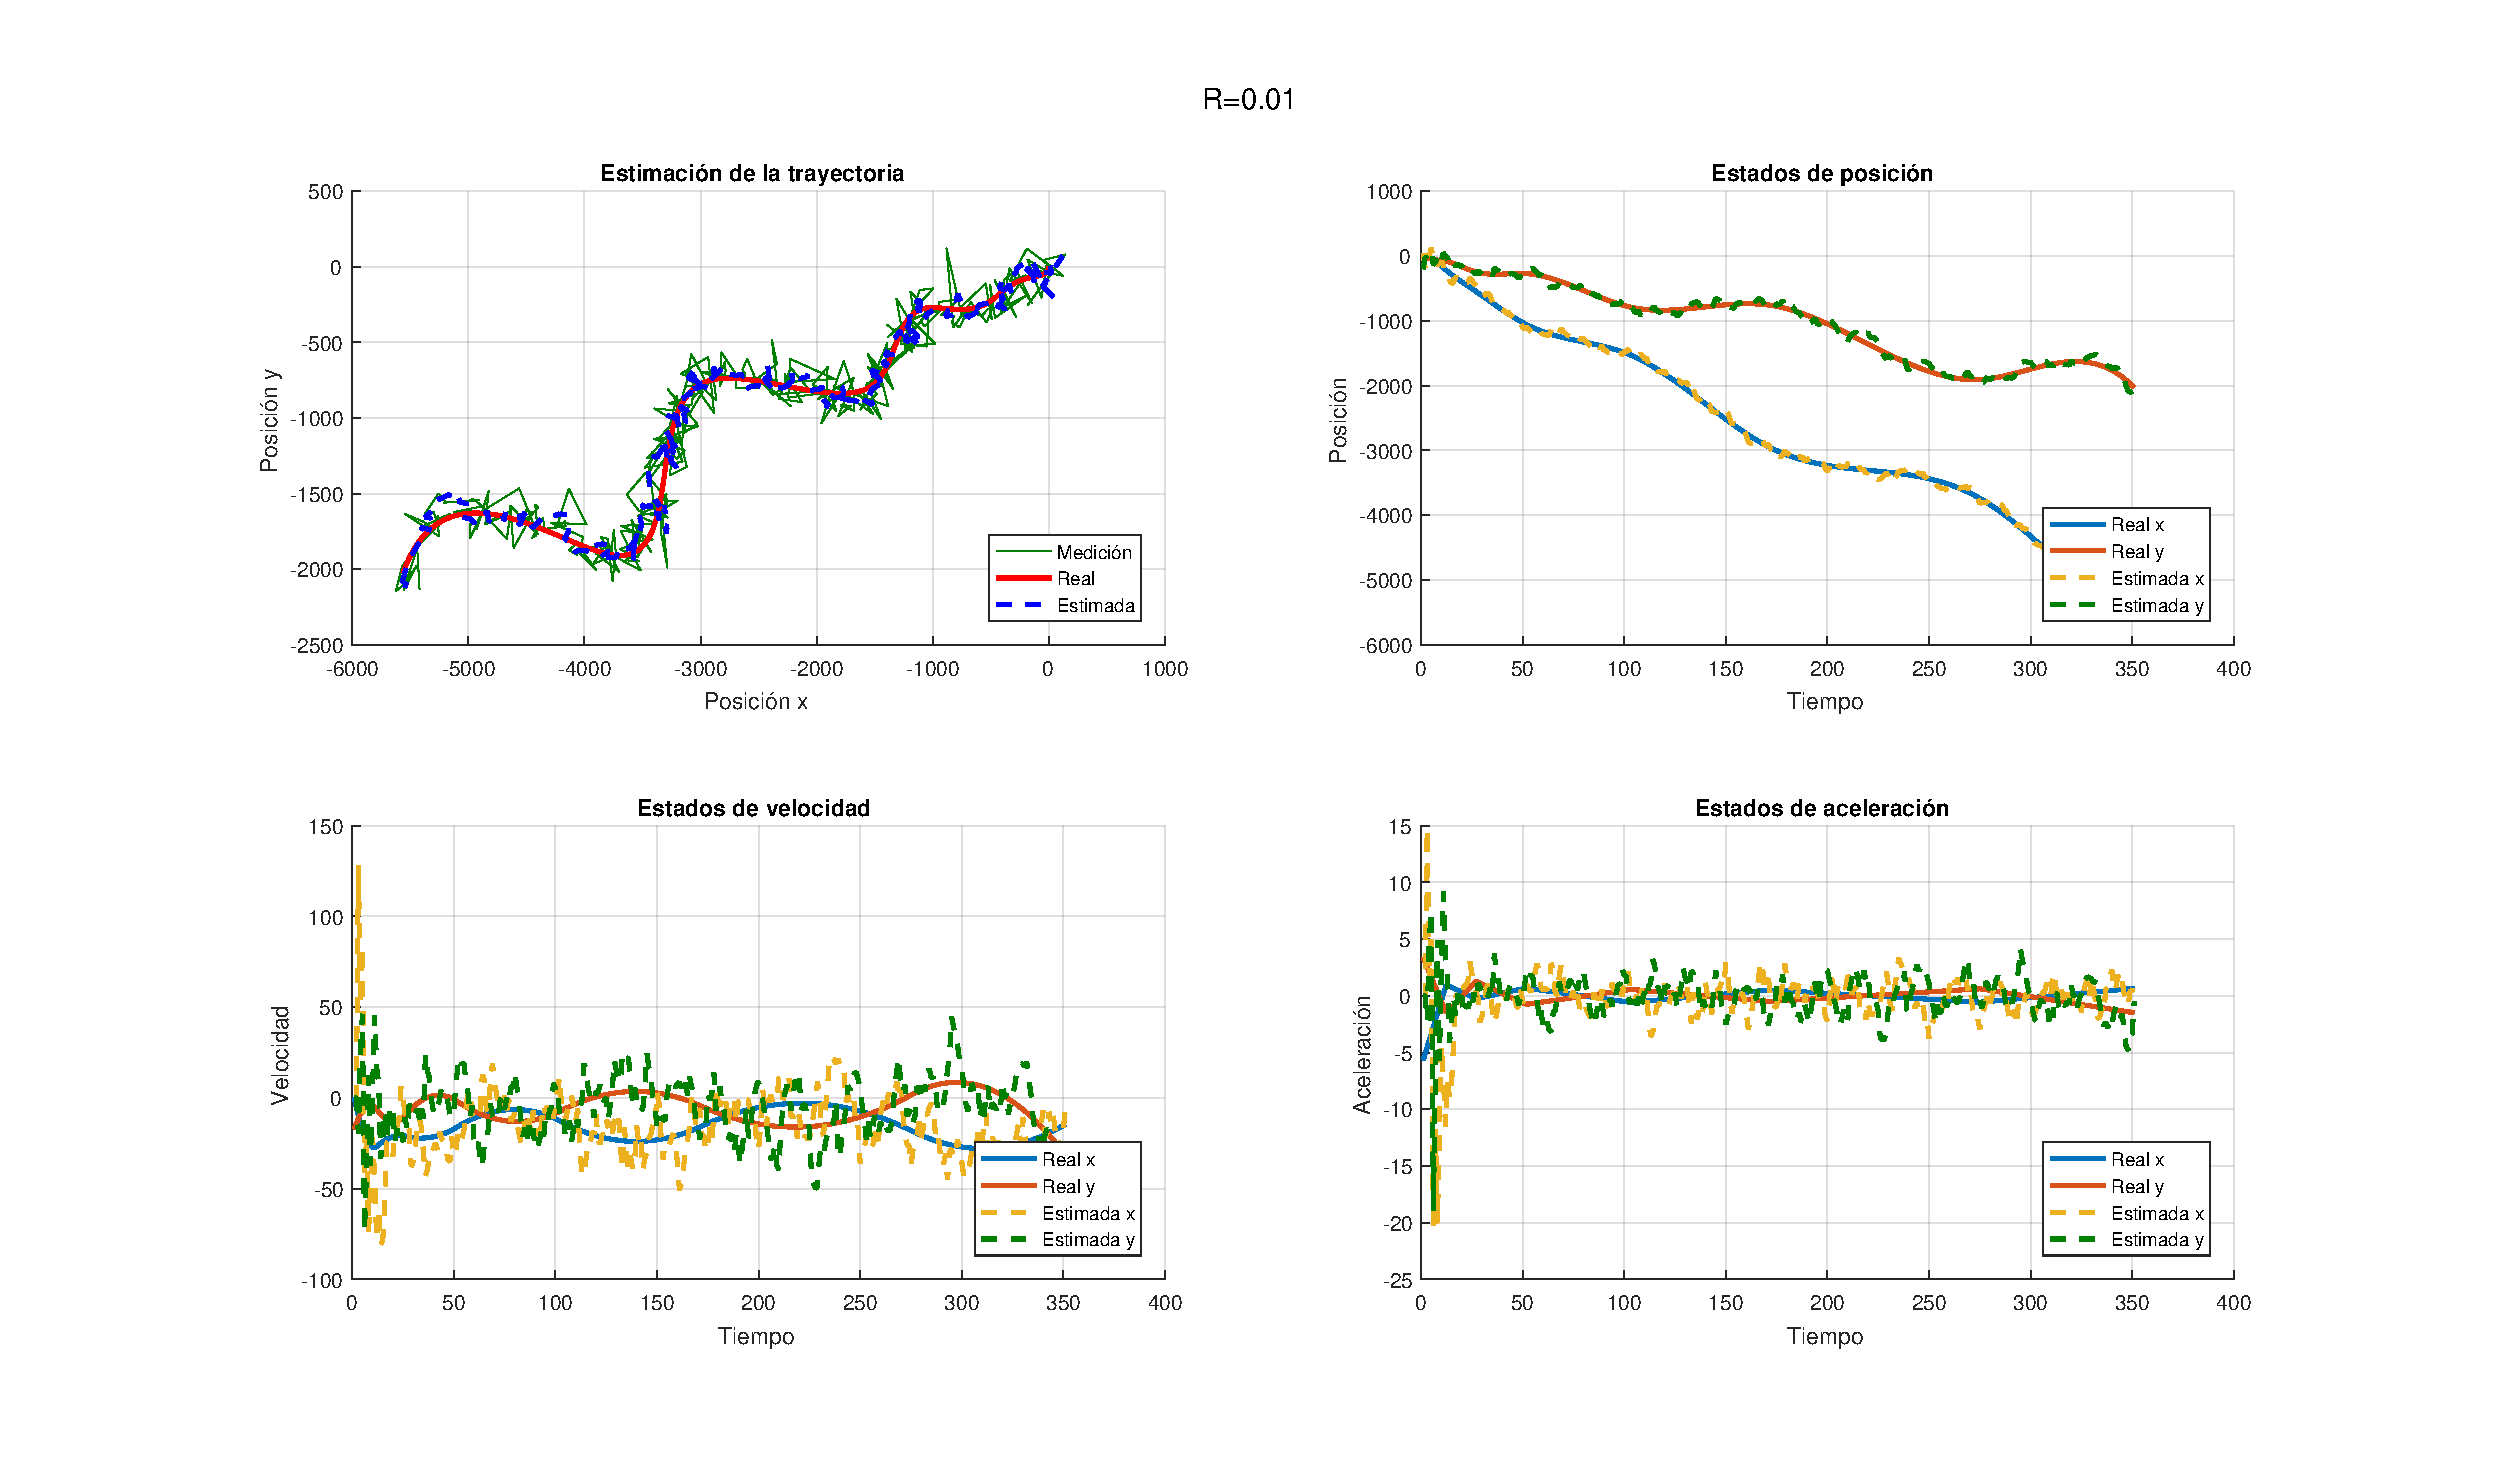
\includegraphics[scale=0.5,trim={6,5cm 0 0 0}]{Figuras/graf_ej6_R2.pdf}
		\caption{Estimación de Trayectoria - Matriz de Covarianza Menor}
		\label{fig:ej5r2}
	\end{figure}
	
	\begin{figure}[H]
		\centering
		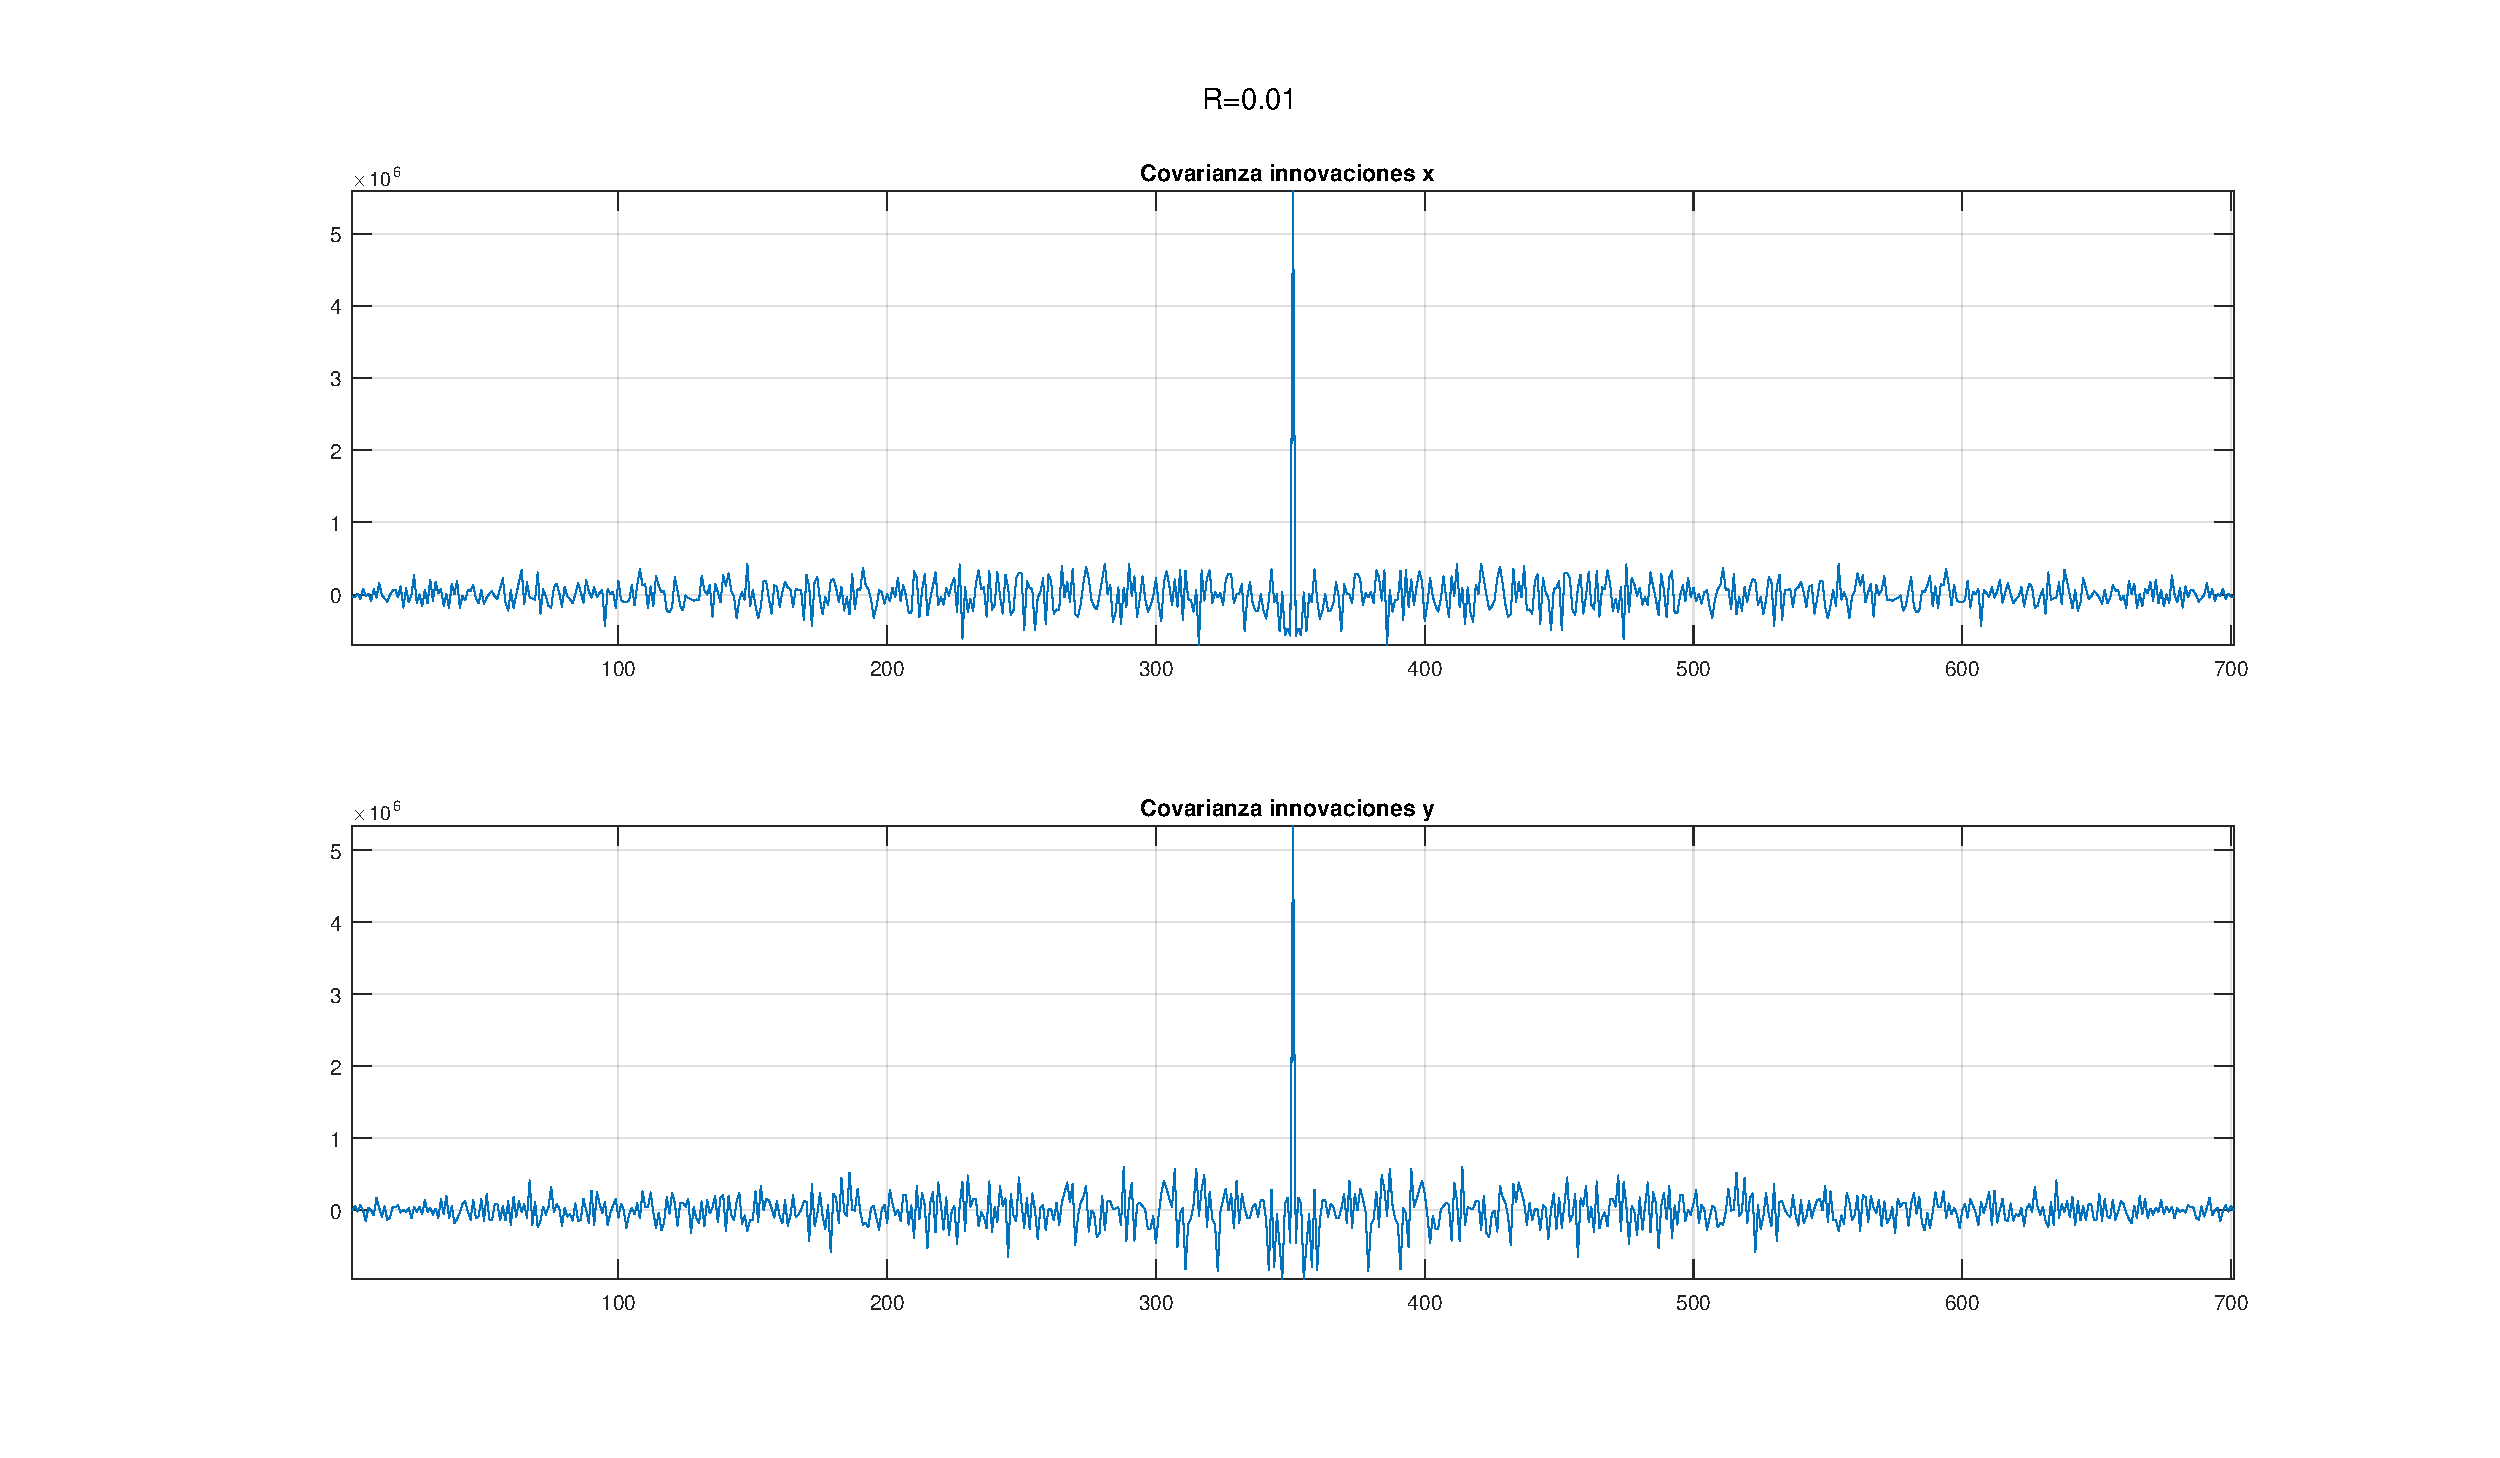
\includegraphics[width=1.0\textwidth,keepaspectratio]{Figuras/covinn_ej6_R2.pdf}
		\caption{Autocorrelación de Innovaciones - Matriz de Covarianza Menor}
		\label{fig:ej5r2_innov}
	\end{figure}
	
	\subsection{Análisis de los resultados}
	En las Figuras \ref{fig:ej5r1} y \ref{fig:ej5r2} se observan las estimaciones de las trayectorias para una matriz de covarianza del ruido de proceso $100$ veces mayor y $100$ veces menor a la original, respectivamente. En el caso de la matriz mayor, el algoritmo le da menos importancia a la dinámica y más a las mediciones. De esta manera, otorga más peso a las mediciones y el error de la trayectoria respecto de la real es mayor que usando una matriz menor. El efecto es similar al presentado en la Sección \ref{sec:ej3}, donde al variar $P$, varía $K$ y en consecuencia se sigue en mayor o menor medida a las mediciones.\\

	Sin embargo, la magnitud de $R$ afecta a la autocorrelación de las innovaciones. En las Figuras \ref{fig:ej5r1_innov} y \ref{fig:ej5r2_innov} se observan las autocorrelaciones de las innovaciones. Cuanto mayor es la matriz de ruido de proceso, el proceso es menos blanco, y por consiguente se concluye que la estimación es peor.


